\documentclass[PublicacaoArtigoOuRelatorio,english,portuguese,LogoINPE]{tdiinpe}


%%%%%%%%%%%%%%%%%%%%%%%%%%%%%%%%%%%%%%%%%%%%%
%%% Pacotes j� previamente carregados:      %
%%%%%%%%%%%%%%%%%%%%%%%%%%%%%%%%%%%%%%%%%%%%%%%%%%%%%%%%%%%%%%%%%%%%%%%%
%%% ifthen,calc,graphicx,color,inputenc,babel,hyphenat,array,setspace, %
%%% bigdelim,multirow,supertabular,tabularx,longtable,lastpage,lscape, %
%%% rotate,caption2,amsmath,amssymb,amsthm,subfigure,tocloft,makeidx,  %
%%% eso-pic,calligra,hyperref,ae,fontenc                               %
%%%%%%%%%%%%%%%%%%%%%%%%%%%%%%%%%%%%%%%%%%%%%%%%%%%%%%%%%%%%%%%%%%%%%%%%
\usepackage{siunitx}
\usepackage{dsfont}
\usepackage{comment}

%ADICOINAIS%%%%%%%%%%%%%%%%%%%%%%%%%%%%%%%%%%%%%%%%%%%%%
\usepackage{rotating}
\usepackage{amssymb}
\usepackage{bm}
\usepackage{color}
\usepackage{colortbl}
\usepackage{mathrsfs}
\usepackage{enumerate}
\usepackage[section]{placeins}

\DeclareMathOperator*{\argmax}{arg\,max}
\DeclareMathOperator*{\argmin}{arg\,min}
\DeclareMathOperator*{\maxi}{max}
\DeclareMathOperator*{\mini}{min}
\DeclareMathOperator*{\sgn}{sgn}

%\usepackage{natbib}

\usepackage{pdfpages}

%\renewcommand{\labelenumi}{\arabic{enumi}.}
\renewcommand{\thefootnote}{(\arabic{footnote})}

%\makeatletter
%\newcommand{\thickhline}{\noalign {\ifnum 0=`}\fi \hrule height 1pt \futurelet \reserved@a \@xhline}
%\newcolumntype{"}{@{\hskip\tabcolsep\vrule width 1pt\hskip\tabcolsep}}
%\makeatother
%%%%%%%%%%%%%%%%%%%%%%%%%%%%%%%%%%%%%%%%%%%%%%%%%%%%%%%%



%%%%%%%%%%%%%%%%%%%CAPA%%%%%%%%%%%%%%%%%%%%%%%%%%%%%%%%
%\serieinpe{INPE-NNNNN-TDI/NNNN} %% n�o mais usado

%\titulo{CARACTERIZA��O DAS DIN�MICAS TEMPORAIS DO USO E COBERTURA DO SOLO EM �REAS DO PANTANAL AFETADAS PELAS QUEIMADAS RECENTESNO ANO DE 2020}
\titulo{FLOODING FORECAST VIA INTEGRATION
OF TWEETS, WEATHER DATA AND
MACHINE LEARNING ALGORITHMS}

\title{}
\author{Student: Vitor Yuichi Hossaki \\ Supervisor: Prof. Dr. Leonardo Bacelar Lima Santos}
\descriccao{Report to CNPq/Cemaden Scientific Initiation Scholarship Program}
\repositorio{}
\tipoDaPublicacao{}
\IBI{}

\date{Descember of 2021}

%%%%%%%%%%%%%%%%%%%%%%%%%%%VERSO DA CAPA%%%%%%%%%%%%%%%%%%%%%%%%%%%%%%%%%%%%%%%%%%%%%%%
%\tituloverso{\vspace{-0.9cm}\textbf{\PublicadoPor:}}
%\descriccaoverso{%Instituto Nacional de Pesquisas Espaciais - INPE\\
%%Gabinete do Diretor (GB)\\
%%Servi�o de Informa��o e Documenta��o (SID)\\
%%Caixa Postal 515 - CEP 12.245-970\\
%%S�o Jos� dos Campos - SP - Brasil\\
%%Tel.:(012) 3945-6923/6921\\
%%Fax: (012) 3945-6919\\
%%E-mail: {\url{pubtc@sid.inpe.br}}
%}
%
%% CEPPII de 09/12/2011 a 08/12/2013:
%\descriccaoversoA{\textbf{\ConselhoDeEditoracao:}\\
%\textbf{\Presidente:}\\
%Marciana Leite Ribeiro - Servi�o de Informa��o e Documenta��o (SID)\\
%\textbf{\Membros:}\\
%Dr. Antonio Fernando Bertachini de Almeida Prado - Coordena��o Engenharia e Tecnologia Espacial (ETE)\\
%Dr� Inez Staciarini Batista - Coordena��o Ci�ncias Espaciais e Atmosf�ricas (CEA)\\
%Dr. Gerald Jean Francis Banon - Coordena��o Observa��o da Terra (OBT)\\
%Dr. Germano de Souza Kienbaum - Centro de Tecnologias Especiais (CTE)\\
%Dr. Manoel Alonso Gan - Centro de Previs�o de Tempo e Estudos Clim�ticos (CPT)\\
%Dr� Maria do Carmo de Andrade Nono - Conselho de P�s-Gradua��o\\
%Dr. Pl�nio Carlos Alval� - Centro de Ci�ncia do Sistema Terrestre (CST)\\
%\textbf{\BibliotecaDigital:}\\
%Dr. Gerald Jean Francis Banon - Coordena��o de Observa��o da Terra (OBT)\\
%%Jefferson Andrade Ancelmo - Servi�o de Informa��o e Documenta��o (SID)\\
%%Simone A. Del-Ducca Barbedo - Servi�o de Informa��o e Documenta��o (SID)\\
%%Deicy Farabello - Centro de Previs�o de Tempo  e Estudos Clim�ticos (CPT)\\
%\textbf{\RevisaoNormalizacaoDocumentaria:}\\
%Marciana Leite Ribeiro - Servi�o de Informa��o e Documenta��o (SID) \\
%%Maril�cia Santos Melo Cid - Servi�o de Informa��o e Documenta��o (SID)\\
%Yolanda Ribeiro da Silva Souza - Servi�o de Informa��o e Documenta��o (SID)\\
%\textbf{\EditoracaoEletronica:}\\
%Marcelo de Castro Pazos - Servi�o de Informa��o e Documenta��o (SID)\\
%}

%%%%%%%%%%%%%%%%%%%FOLHA DE ROSTO

%%%%%%%%%%%%%%%%FICHA CATALOGR�FICA
%%% N�O PREENCHER - SER� PREENCHIDO PELO SID
%
%\cutterFICHAC{Cutter}
%\autorUltimoNomeFICHAC{Negri, Rog�rio Galante}
%\autorAbreviadoFICHAC {RGN}
%\tituloFICHAC{INVESTIGA��O E DESENVOLVIMENTO DE ALGORITMOS PARA DETEC��O DE MUDAN�A EM IMAGENS DE SENSORIAMENTO REMOTO}
%\instituicaosigla{}
%\instituicaocidade{S�o Jos� dos Campos}
%\paginasFICHAC{\pageref{} + \pageref{}}
%\palavraschaveFICHAC{1.~Palavra chave. 2.~Palavra chave 3.~Palavra chave. 4.~Palavra chave. 5.~Palavra chave  I.~\mbox{T�tulo}.}
%\numeroCDUFICHAC{000.000} %% n�mero do CDU 
%
%% Nota da ficha (para TD)
%\tipoTD{Projeto de Pesquisa}
%\cursoFA{}
%\instituicaoDefesa{}
%\anoDefesa{2013}
%\nomeAtributoOrientadorFICHAC{}
%\valorAtributoOrientadorFICHAC{}
%
%%%%%%%%%%%%%%%%FOLHA DE APROVA�AO PELA BANCA EXAMINADORA
%\tituloFA{\textbf{ATEN��O! A FOLHA DE APROVA��O SER� INCLUIDA POSTERIORMENTE.}}
%%\cursoFA{\textbf{}}
%\candidatoOUcandidataFA{}
%\dataAprovacaoFA{}
%\membroA{}{}{}
%\membroB{}{}{}
%\membroC{}{}{}
%\membroD{}{}{}
%\membroE{}{}{}
%\membroF{}{}{}
%\membroG{}{}{}
%\ifpdf

%%%%%%%%%%%%%%%N�VEL DE COMPRESS�O {0 -- 9}
%\pdfcompresslevel 9
%\fi
%%%% define em 80% a largura das figuras %%%
%\newlength{\mylenfig} 
%\setlength{\mylenfig}{0.8\textwidth}
%%%%%%%%%%%%%%%%%%%%%%%%%%%%%%%%%%%%%%%%%%%%
%
%%%%%%%%%%%%%%%COMANDOS PESSOAIS
%\newcommand{\vetor}[1]{\mathit{\mathbf{#1}}}


\makeindex

\begin{document}

\maketitle

%%\hypertarget{estilo:resumo}{}


\begin{resumo}
%O Vale do Para�ba e Serra da Mantiqueira s�o marcados por grandes transforma��es nos usos e ocupa��o do solo, ao longo dos anos. Tais altera��es constantes na paisagem alteram significativamente a din�mica ambiental do local.  No Vale do Para�ba, especialmente, as transforma��es estiveram vinculadas aos ciclos econ�micos brasileiros que conduziram ao atual cen�rio de grandes concentra��es de plantios de eucaliptos. Devido � proximidade da Serra da Mantiqueira em rela��o ao Vale do Para�ba, as altera��es nos usos e coberturas do solo nesta regi�o sofrem influ�ncia do crescimento populacional e industrial.  Neste contexto, estudos temporais sobre uso e cobertura do solo permitem observar modifica��es e avaliar os impactos gerados por elas. Tendo em vista a relev�ncia de an�lises desta natureza para o monitoramento e gest�o ambiental, o presente projeto objetiva estudar os efeitos da silvicultura no uso e cobertura do solo nas regi�es do Vale do Para�ba e Serra da Mantiqueira, atrav�s de an�lises de detec��o de mudan�as sobre a din�mica de expans�o da silvicultura nos anos de 1987, 1997, 2007 e 2017. Ser�o utilizadas imagens LANDSAT-5 TM e LANDSAT-8 OLI para uma an�lise em macroescala e determina��o de atores respons�veis pela mudan�a na paisagem da �rea de estudo. Atrav�s de imagens RapidEye, regi�es de maior relev�ncia ou impacto na mudan�a da paisagem ser�o analisadas em microescala, possibilitando melhores an�lises, reflex�es e conclus�es sobre o fen�meno estudado.
\end{resumo}

%Classifica��o de imagens de Sensoriamento Remoto � uma das mais importantes aplica��es de Reconhecimento de Padr�es em estudos ambientais. A import�ncia de se obter resultados de classifica��o cada vez mais precisos motiva progressivamente o desenvolvimento e o aprimoramento das t�cnicas de classifica��o de imagens. 

\includeSumario
\inicioIntroducao

\doublespacing


\chapter{INTRODU��O}\label{intro}

%Abertura e motiva��o...
Recentemente, o Brasil tem enfrentado uma s�rie de impactos imensur�veis ao meio ambiente e � sua biodiversidade, assim como danos sociais e econ�micos.
Exemplos recentes contemplam o rompimento de barragens de rejeito de min�rio, desmatamentos e inc�ndios florestais.


A regi�o do Pantanal Mato-grossense possui uma das maiores plan�cies de inunda��o do mundo, por�m, � caracterizada por um per�odo de estiagem muito forte entre os meses de junho a agosto. Nesse per�odo, os fazendeiros locais costumam atear fogo para ampliar as zonas de pasto e possibilitar o crescimento acelerado da produ��o pecu�ria \cite{AraujoSilva2015}. Atualmente, a regi�o do Pantanal, vive a maior seca desde a d�cada de 1970 que, atrelada com o efeito do uso do fogo, � respons�vel pelas maiores queimadas da hist�ria do local. Segundo \cite{MoraesEA2017}, esse tipo de fen�meno pode apresentar diversos efeitos ambientais negativos que v�o desde a perda da biodiversidade at� fortes impactos nos sistemas clim�ticos e terrestres.


%Uso do SR -- amplas areas e multitemporal
Eventos como estes motivam a elabora��o de estudos capazes de auxiliar no entendimento e monitoramento sistem�tico de �reas que implicam riscos � sociedade e ao meio ambiente.
Neste contexto, o sensoriamento remoto surge como uma tecnologia de extrema utilidade, uma vez que permite an�lises amplas no espa�o e de forma multitemporal.


%T�cnicas...
No �mbito do desenvolvimento de ferramentas de monitoramento, as t�cnicas de classifica��o e regress�o de dados \cite{Geron2019}, bem como uso de m�tricas espaciais \cite{herold2002} para caracteriza��o do dom�nio espacial, destacam-se como outra componente de grande import�ncia.
Quando aliadas aos dados obtidos por sensoriamento remoto, tais t�cnicas viabilizam a extra��o de conhecimento da superf�cie terrestre de forma automatizada.


%Ideia do que ser� feito...
Em face a esta problem�tica, este projeto de pesquisa prop�e analisar as din�micas de uso e cobertura do solo em uma regi�o do pantanal e, por meio de um modelo de regress�o, verificar rela��es desempenhadas por tais din�micas sobre a ocorr�ncia, ou n�o, de inc�ndios. O modelo de regress�o mencionado surge como ferramenta para o mapeamento de �reas suscet�veis a inc�ndios.


%Organiza��o do texto
O texto a seguir est� organizado da seguinte forma: na Se��o~\ref{Obj} � enunciado o objetivo geral e listados os objetivos espec�ficos do projeto; justificativas e relev�ncias desta pesquisa s�o expostas na Se��o~\ref{Jus}; uma breve discuss�o sobre m�todos de classifica��o e regress�o de dados bem como sobre m�tricas espaciais � apresentada na Se��o~\ref{Rev}; a Se��o~\ref{Proposta} � reservada para exposi��o e discuss�o da proposta de pesquisa em si; na Se��o~\ref{MatMet} � apresentada uma descri��o da �rea de estudo e dos dados dispon�veis, assim como sobre os procedimento metodol�gicos a serem realizados; por fim, � delineada uma concep��o de como a pesquisa proposta dever� ser desenvolvida, seguido de um cronograma de atividade, exposto na Se��o~\ref{Cron}.




\chapter{OBJETIVOS}\label{Obj}

Este projeto de pesquisa tem como objetivo principal investigar as din�micas de mudan�a no uso e cobertura do solo em de regi�es inseridas no Pantanal Mato-grossense, no per�odo de 2000 a 2019, e que posteriormente foram afetadas pelos inc�ndios recentes ocorridos no ano de 2020. 
Tal investiga��o ser� fomentada por dados multitemporais obtidos por sensoriamento remoto e por t�cnicas de Processamento Digital de Imagens e Aprendizado de M�quina.


Como objetivos espec�ficos, s�o delineados:

{%\singlespace
\begin{enumerate}%[i --]
\item Implementa��o de procedimento para caracteriza��o das din�micas temporais sobre o uso e cobertura do solo;

\item Aplica��o do procedimento implementado sobre uma s�rie hist�rica de imagens Landsat compreendida entre os anos de 2000 e 2019 em uma �rea de estudo espec�fica;

\item An�lise e caracteriza��o das din�micas do comportamento das �reas afetadas ou n�o pelos inc�ndios recentes;

\item Publica��o dos resultados obtidos em eventos ou peri�dicos cient�ficos.
\end{enumerate}
}    %ok!

%\chapter{JUSTIFICATIVA E RELEV�NCIA DO PROJETO} \label{Jus}


O projeto tem relev�ncia nas �reas ambiental e computacional. No ponto de vista ambiental, o projeto apresentar� uma investiga��o multitemporal sobre as din�micas no uso e cobertura do solo e os inc�ndios recentes na regi�o do Pantanal Mato-grossense. Com isso, vislumbra-se identificar rela��es entre as itera��es antr�picas e o meio atingido pelos inc�ndios.

Em rela��o ao vi�s computacional, este projeto visa desenvolver uma metodologia que converte uma s�rie temporal de imagens de sensoriamento remoto em um descritor sobre as itera��es no uso e cobertura do solo, que por sua vez torna-se �til na constru��o de modelo de previs�o/regress�o capaz de avaliar a suscetibilidade de outras regi�es vizinhas � inc�ndios.


 %ok!

\chapter{FUNDAMENTA��O TE�RICA}\label{Rev}


%%%%%%%%%%%%%%%%%%%%%%%%%%%%%%%%%%%%%%%%%%%%%%%%%%%%%
\section{Classifica��o e regress�o}\label{revClassRegress}

Estudos em Sensoriamento Remoto com foco na classifica��o de imagens tem atra�do a aten��o da comunidade cient�fica, pois os resultados provenientes destas t�cnicas servem de base para diversas aplica��es ambientais e socioecon�micas. 
%Por�m, a classifica��o de imagens de Sensoriamento Remoto, de forma a criar um mapa tem�tico � um desafio, uma vez que a complexidade da paisagem, a escolha da imagem, o processamento e abordagem de classifica��o podem afetar o sucesso do procedimento. 
Sua import�ncia t�m motivado ainda o desenvolvimento de novas propostas capazes de proporcionar resultados de classifica��o cada vez mais acurados \cite{lu2007}.

Um classificador � representado por uma fun��o $F: \mathcal{X} \rightarrow \mathcal{Y}$ , que associa elementos do espa�o de atributos $\mathcal{X}$ a uma das classes de $\Omega = \left\{ \omega_{1}, \omega_{2}, \ldots, \omega_{c}\right\}$, com $c \in \mathbb{N}^{*}$, a partir de um dado r�tulo (indicador) de classe em $\mathcal{Y} = \left\{ 1,2,\ldots,c\right\}$. Nestas condi��es, para $\textbf{x} \in \mathcal{X}$ e $y \in \mathcal{Y}$, $y = F(\textbf{x})$ indica que $\textbf{x}$ pertence � classe $\omega_{y}$.

A classifica��o de imagens consiste na aplica��o de $F$ sobre os vetores de atributos dos pixels (padr�es) que comp�em uma imagem $\mathcal{I}$, definida sobre um reticulado (suporte) $\mathcal{S} \subset \mathbb{N}^{2}$, cujo resultado de classifica��o pode ser denotado por $F(\mathcal{I})$. Com rela��o � imagem em que � conduzido o processo de classifica��o, $\mathcal{I}(s) = \mathbf{x}$, denota que o pixel $s \in \mathcal{S}$ de $\mathcal{I}$ possui atributos representados pelo vetor $\mathbf{x} \in \mathcal{X}$, ainda $C(s) = \omega_{y}$ tal que $F(\textbf{x})=y$.

Os diferentes m�todos de classifica��o de imagem propostos na literatura podem ser entendidos como maneiras distintas de modelar a fun��o $F: \mathcal{X} \rightarrow \mathcal{Y}$ e aplic�-la na classifica��o de $\mathcal{I}$. Os paradigmas supervisionado e n�o supervisionado s�o duas formas/abordagens usualmente adotadas pelos m�todos de classifica��o de imagens. No aprendizado supervisionado s�o fornecidos ao m�todo um conjunto de exemplos de treinamento $\mathcal{D} = \left\{ (\mathbf{x}_{i}, y_{i})\in \mathcal{X} \times \mathcal{Y} : i = 1,2,\ldots,m \right\}$ composto por $m \in \mathbb{N}^{*}$ vetores, onde seus respectivos r�tulos da classe associada s�o conhecidos. Ent�o, o mapeamento entre $\mathcal{X}$ e $\mathcal{Y}$ definido por $F$ representa o conhecimento adquirido das informa��es observadas em $\mathcal{D}$. %No aprendizado n�o supervisionado, os dados s�o analisados pelo algoritmo, a fim de definir agrupamentos sobre os mesmos \cite{monard2003}.
M�todos como M�quina de Vetores Suporte e Florestas Aleat�rias t�m mostrado efici�ncia na classifica��o de imagens de sensoriamento remoto \cite{LiEA2014}.



Em analogia aos m�todos de classifica��o, um modelo de regress�o abrange a
obten��o de uma fun��o $G:\mathcal{X} \rightarrow \mathbb{R}$, que uma vez modelada atrav�s de um conjunto de observa��es $\mathcal{D} = \left\{ (\mathbf{x}_{i}, y_{i})\in \mathcal{X} \times \mathbb{R} : i = 1,2,\ldots,m \right\}$, permite extrapolar valores reais face a um dado vetor de atributos.
Dentre diversos modelos existentes na literatura, a Regress�o Log�stica, tem sido amplamente empregada na estima��o da probabilidade de pertin�ncia ``elemento-classes'' em casos de associa��o bin�ria (i.e., envolvendo apenas duas classes) \cite{Geron2019}, o qual pode ser entendido como uma composi��o entre as fun��o linear e sigmoide, ou seja:
\begin{equation}\label{eqC9ModLogit}
g(\mathbf{x};\mathbf{\theta}) = \frac{1}{1+e^{-\left( \mathbf{\theta}^T \mathbf{x} \right)}}.
\end{equation}



Devido a sua estrutura sigmoide, possui imagem definida sobre o intervalo $[0,1]$. No contexto dos problemas de classifica��o\footnote{As classes mencionadas podem ser interpretadas como ``aus�ncia'' ou ``presen�a'' de determinada caracter�stica.}, $g(\mathbf{x}_i;\mathbf{\theta}) < 0,5$ implica que $\mathbf{x}_i$ deve pertencer � classe de indicador $0$; analogamente, dever� estar associado � classe de indicador $1$ quando $g(\mathbf{x}_i;\mathbf{\theta}) \geq 0,5$. Ainda, � poss�vel interpretar os resultados gerados como uma ``probabilidade de pertin�ncia'' que migra gradativamente entre duas condi��es opostas.


%%%%%%%%%%%%%%%%%%%%%%%%%%%%%%%%%%%%%%%%%%%%%%%%%%%%%
\section{M�tricas espaciais}\label{revMetricas}

M�tricas espaciais s�o medidas derivadas da an�lise digital de mapas a fim de quantificar a heterogeneidade espacial em uma determinada escala e resolu��o \cite{herold2002}. Tais medidas permitem caracteriza��es quantitativas sobre a composi��o espacial, configura��es do \textit{habitat} e dos tipos de cobertura do solo. %A combina��o do Sensoriamento Remoto com m�tricas espaciais podem ser �teis na obten��o de informa��es consistentes e detalhadas sobre a estrutura urbana, possibilitando assim maior representa��o e melhor entendimento do processo de crescimento urbano \cite{deng2009}.
%Como instrumentos de an�lise sobre a constitui��o da paisagem, v�m-se adotando as m�tricas espaciais como mecanismos de compreens�o das implica��es do crescimento urbano. 
Por meio destas medidas, � poss�vel identificar estruturas, padr�es e conectividade de �reas, e ainda, o n�mero, tamanho, forma e proximidade das manchas de uso e cobertura do solo.
%, avaliando os impactos de poss�veis expans�es de cidades \cite{lee2011}.
%Nesta pesquisa � proposto o uso das m�tricas espaciais denominadas por porcentagem de cobertura, coeficiente de varia��o das �reas das manchas, densidade de manchas e densidade de bordas.
Quatro tipos de m�tricas espaciais mostram-se �teis na caracteriza��o do espa�o, s�o elas: porcentagem de cobertura, coeficiente de varia��o das �reas das manchas, densidade de manchas e densidade de bordas.

Inicialmente, para a defini��o de mancha � observada uma vizinhan�a espacial, definida por:
\begin{equation}\label{vizinhos}
\mathcal{V}_{\rho}\left(s_{i}\right) = \left\{ s_{i} \in \mathcal{S} : d\left( s_{i},t\right) < \rho; t \in \mathcal{S} \right\},
\end{equation}
sendo $d(\cdot ,\cdot)$ a dist�ncia do m�ximo, isto �: $d\left( a, b \right) = \max\left\{ \left| a_{1} - b_{1} \right|, \left| a_{2} - b_{2} \right| \right\}$ para $a = \left\{ a_{1}, a_{2} \right\}$ e $b = \left\{ b_{1}, b_{2} \right\}$ elementos de $\mathcal{S}$. Ainda, $\rho$ representa o raio de vizinhan�a de $s_{i}$.

Uma vez definida a vizinhan�a de $s_{i}$, s�o identificadas como manchas cada conjunto de posi��es que apresentam classe comum e s�o espacialmente conectadas segundo uma vizinhan�a de ordem 1 (\textit{i.e.}, vizinhan�a-4). Formalmente, uma mancha $M^{(y)}_{j}\left( s_{i}, \rho \right)$ � o conjunto representado por:

\begin{equation}\label{manchas}
M^{(y)}_{j}\left( s_{i}, \rho \right) = \left\{ t \in \mathcal{V}_{\rho}(s_{i}) : C(t) = \omega_{y}, C(t)=C(r), \left\| t-r \right\| \leq 1 \right\}.
\end{equation}

A porcentagem de cobertura que representa a propor��o de cada classe sobre a �rea total, � expressa por:
\begin{equation}\label{pctcbrtr}
P_{y} = \frac{A_{y}}{A},
\end{equation}
onde $A_{y} = \#\bigcup\limits^{m_{y}}_{j=1}M^{(y)}_{j}\left( s_{i}, \rho \right)$ representa a �rea das manchas associadas � classe $\omega_{y}$, dada pelo total de pixels associados a esta classe, e $A = \#\bigcup\limits^{c}_{k=1} \bigcup\limits^{m_{k}}_{j=1}M^{(k)}_{j}\left( s_{i}, \rho \right)$ determina a soma das �reas de todas as manchas. Ainda, $m_{k}$ representa o n�mero de manchas relacionadas a uma dada classe $\omega_{k} \in \Omega$.

O coeficiente de varia��o das manchas, por ser expresso em porcentagem, permite comparar a varia��o das �reas das manchas entre diferentes classes. Tal coeficiente � expresso por:
\begin{equation}\label{coefvar}
CV_{y} = \frac{\sigma\left( M^{(y)}_{j}\left( s_{i}, \rho \right) \right)}{\mu\left( M^{(y)}_{j}\left( s_{i}, \rho \right) \right)}; \ j=1, \ 2, \ \dots, \ m_{y} \ ,
\end{equation}
onde $CV_{y}$, $\sigma\left( M^{(y)}_{j}\left( s_{i}, \rho \right) \right)$ e $\mu\left( M^{(y)}_{j}\left( s_{i}, \rho \right) \right)$ s�o, respectivamente, o coeficiente de varia��o, desvio padr�o e m�dia das �reas das manchas associadas � classe $\omega_{y}$ referente a vizinhan�a $\mathcal{V}_{\rho}\left(s_{i}\right)$.

A densidade de manchas quantifica a propor��o do n�mero de manchas de determinada classe em rela��o � �rea de todas as manchas. Tal m�trica � dada por:
\begin{equation}\label{denman}
D_{y} = \frac{m_{y}}{A},
\end{equation}

Por fim, densidade de bordas quantifica a propor��o do comprimento das bordas em rela��o � �rea de todas as manchas, dado por:
\begin{equation}\label{denbor}
B_{y} = \frac{\sum\limits^{m_{y}}_{j=1}b^{(y)}_{j}\left( s_{i}, \rho \right)}{A},
\end{equation}
onde $b^{(y)}_{j}$ corresponde ao per�metro de uma mancha $M^{(y)}_{j}\left( s_{i}, \rho \right)$.



%%%%%%%%%%%%%%%%%%%%%%%%%%%%%%%%%%%%%%%%%%%%%%%%%%%%%
\section{Breve discuss�o sobre Florestas Aleat�rias}\label{revRF}


Florestas Aleat�rias ({\itshape Random Forest} -- RF) \cite{Breiman2001} compreende uma abordagem de classifica��o que combina um conjunto de �rvores de decis�o. Dois pontos importantes desta abordagem referem-se ao uso da amostragem {\itshape bootstrap} na determina��o de conjuntos de dados de treinamento e da vota��o por maioria para a tomada de decis�o final.

Diante do fato das �rvores de decis�o serem sens�veis aos dados de treinamento, os modelos obtidos tendem a apresentar certo grau de distin��o entre si. Como consequ�ncia, durante o processo de classifica��o uma �rvore dever� proteger outra �rvore do seu pr�prio erro, logo, a classifica��o ocorre de forma err�nea somente quando as �rvores erram em favor de uma mesma classe.

Outro fator que aumenta ainda mais a distin��o entre as �rvores � a sele��o aleat�ria de apenas parte dos atributos dispon�veis para uso em cada uma das �rvore que comp�e a combina��o. 
Uma vez que a combina��o das decis�es � tomada com base na vota��o por maioria, espera-se que uma grande quantidade de modelos parcialmente distintos deve superar, em opini�o, um �nico modelo constituinte.

%As caracter�sticas mencionadas torna o RF um dos m�todos de Aprendizado de M�quina mais robustos dentro desta �rea de pesquisa.


%\hypertarget{estilo:capitulo}{}
%%%%%%%%%%%%%%%%%%%%%%%%%%%%%%%%%%%%%%%%%%%%%%%%%
\chapter{MODELAGEM DA SUSCETIBILIDADE � INC�NDIOS} \label{Proposta}

O diagrama ilustrado na Figura~\ref{framework} cont�m o racional desta proposta de pesquisa. Seus diferentes constituintes compreendem os conceitos discutidos na Se��o~\ref{Rev}.

%%%%%%%%%%%%%%%%%%%%%%%%%%%%%%
\begin{figure}[h!]
\centering
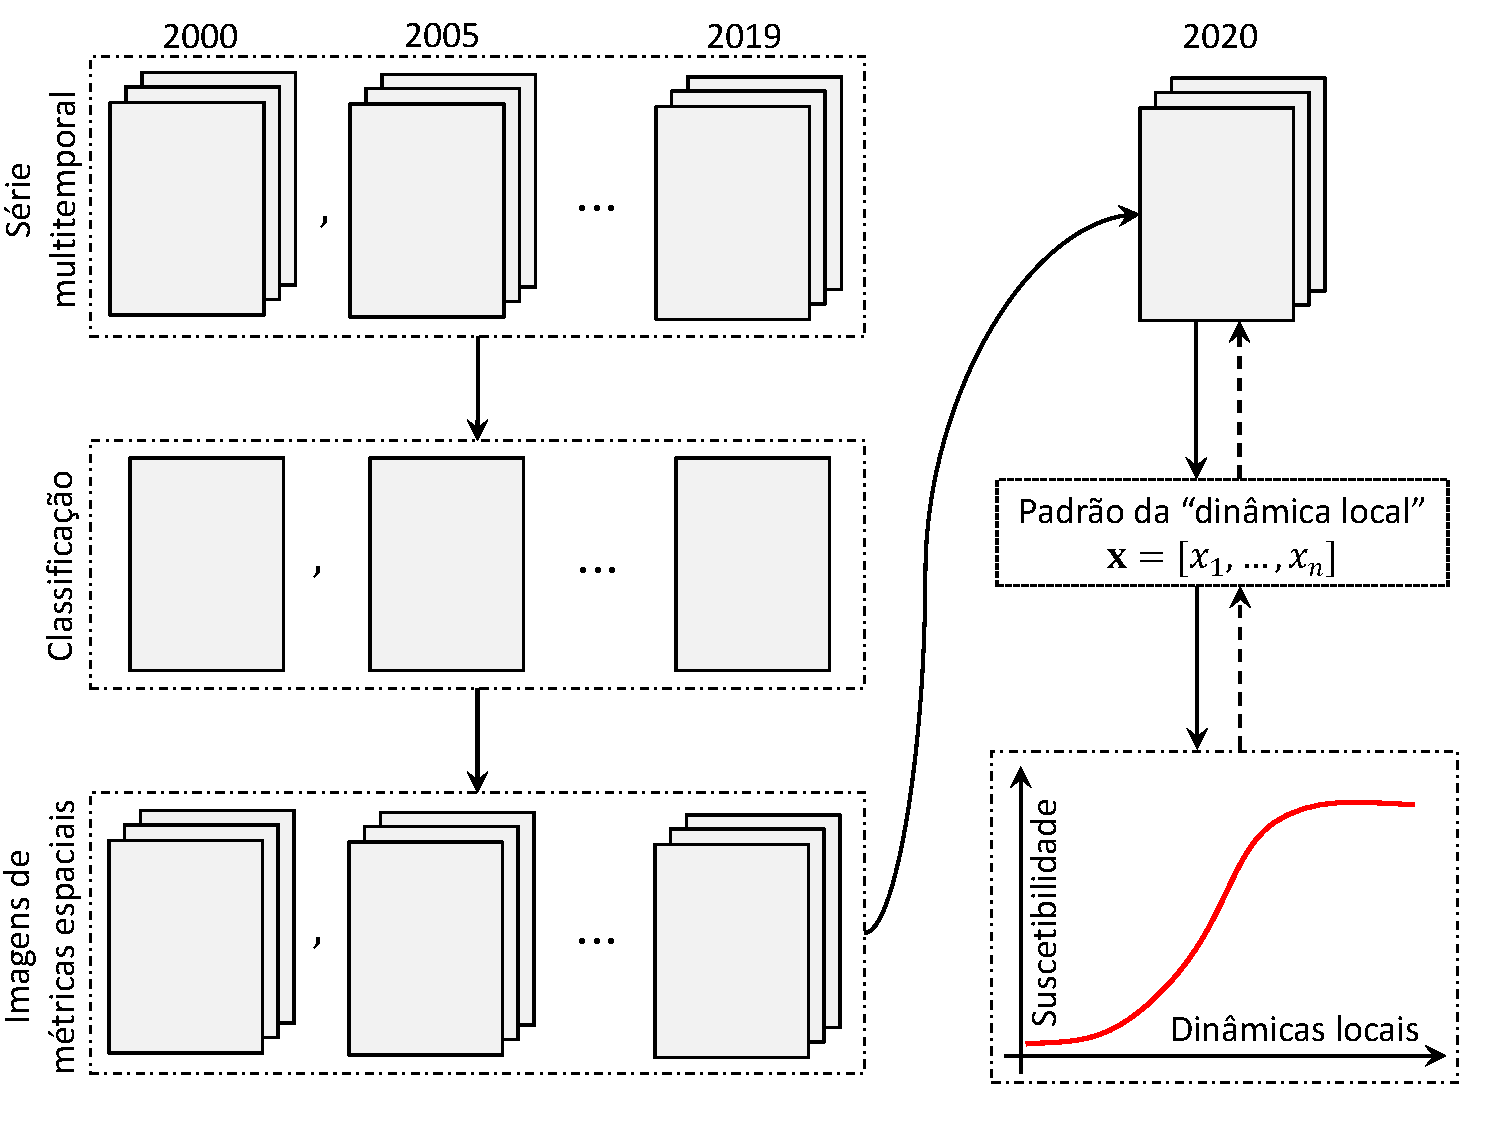
\includegraphics[width=\textwidth]{./figs/FrameworkProjFelipeNascimento.pdf}
\caption{Racional da proposta de pesquisa.}\label{framework}
\end{figure}

Partindo de uma s�rie multitemporal de imagens obtidas por sensoriamento remoto, especificamente compreendida pelos anos de 2000, 2005, 2010, 2015 e 2019\footnote{Tais anos est�o pass�veis de modifica��o perante situa��es extremas, por exemplo, a cobertura de nuvem ou aus�ncia de dados.}. Sobre cada uma destas imagens � efetuada a sele��o de amostras de uso e cobertura do solo dentre quatro classes poss�veis: alta biomassa; m�dia biomassa; baixa biomassa; outros. Ao passo que a classe de baixa bomassa corresponde a �reas de solo exposto ou agropastoril, as classes de alta e m�dia biomasssa correspondem a locais de floresta e regenera��o recente. A quarta classe, denominada ``outros'' � destinada a corpos d'�gua e demais alvos cujo ac�mulo de biomassa � improv�vel.

Posteriormente, cada uma das imagens da s�rie multitemporal, devidamente acompanhada das amostras de uso e cobertura do solo, � ent�o submetida a um processo de classifica��o com uso do m�todo RF (Se��o~\ref{revRF}). A parametriza��o e avalia��o dos resultados de classifica��o � guiado por procedimento {\itshape grid-search} e avalia��es via coeficiente kappa \cite{CongaltonGreen2009}.

Em posse dos resultados de classifica��o, ser�o aplicadas m�tricas espaciais para extra��o e caracteriza��o das din�micas locais em um espa�o de atributos de dimens�o elevada. Ao admitir as quatro m�tricas\footnote{Supondo um valor fixo para o raio de vizinhan�a ($\rho$)} discutidas na Se��o~\ref{revMetricas} (Equa��es~\ref{pctcbrtr} a \ref{denbor}) e que a s�rie multitemporal possui quatro instantes (i.e., 2000, 2005, 2010, 2015 e 2019), � proporcionado ao fim uma imagem cujos pixels est�o associados a um vetor de dimens�o 20.

Por sua vez, com referencia em uma imagem recente da �rea de estudo, � efetuada a coleta de amostras sobre regi�es afetadas, ou n�o, por inc�ndios. Este processo leva a composi��o de um conjunto rotulado das din�micas locais. Com uso deste conjunto � viabilizada a determina��o de um modelo de regress�o log�stica, que por sua vez pode ser empregado na extrapola��o do comportamento ``afetadas'' e ``n�o afetadas'' como fun��o das din�micas locais.

O modelo de regress�o obtido, quando aplicado sobre �reas n�o rotuladas, ou mesmo sobre regi�es vizinhas da �rea de estudo que tenham sido submetidas ao mesmo processo de classifica��o e extra��o de m�tricas espaciais, deve proporcionar uma infer�ncia a respeito da suscetibilidade a inc�ndios. A avalia��o deste processo pode ser feito mediante a compara��o entre a estima��o gerada pelo modelo obtido em locais onde � conhecida a ocorr�ncia, ou n�o, de inc�ndios. Mais uma vez, o coeficiente kappa deve ser empregado neste prop�sito de avalia��o.

     %fazer

%\hypertarget{estilo:capitulo}{}

\chapter{MATERIAIS E M�TODOS} \label{MatMet}

%%%%%%%%%%%%%%%%%%%%%%%%%%%%%%%%%%%%%%%%%%%%%%%%%
\section{�rea de estudo e dados dispon�veis} \label{AreaEstudo}


Nos limites da �rea de estudo, ilustrada na Figura~\ref{areaestudo}, est� inserido o munic�pio de C�ceres, estado do Mato-Grosso, que abrange aproximadamente 24,6 mil quil�metros quadrados de extens�o. Este munic�pio comp�e a regi�o Centro-Sul Mato-grossense e � divido em tr�s biomas predominantes: Amaz�nia, Cerrado e o Pantanal. Dentre os tr�s biomas citados anteriormente, o Pantanal � o bioma mais expressivo no munic�pio de C�ceres, ocupando cerca de 51\% de sua �rea total \cite{IBGE2020}.

A regi�o apresenta uma temperatura m�dia anual de 26,4 ${}^{\textrm{o}}\textrm{C}$ e precipita��o anual m�dia de 1,335 mil�metros. Estas caracter�sticas comp�em um clima baseado em duas esta��es bem definidas, um per�odo quente e �mido, que ocorre entre dezembro e mar�o, e um per�odo de seca que dura de abril a novembro \cite{NevesEA2012}. Ultimamente a regi�o do pantanal Mato-grossense enfrenta um per�odo de seca intensa que, somado com o efeito do uso do fogo, registra 2020 como o ano com maior n�mero de focos de inc�ndio da hist�ria desde 1998\footnote{https://observatoriopantanal.org/2020/07/21/pantanal-bate-recorde-historico-de-queimadas-em-22-anos/}.


\begin{figure}[ht!]
\centering
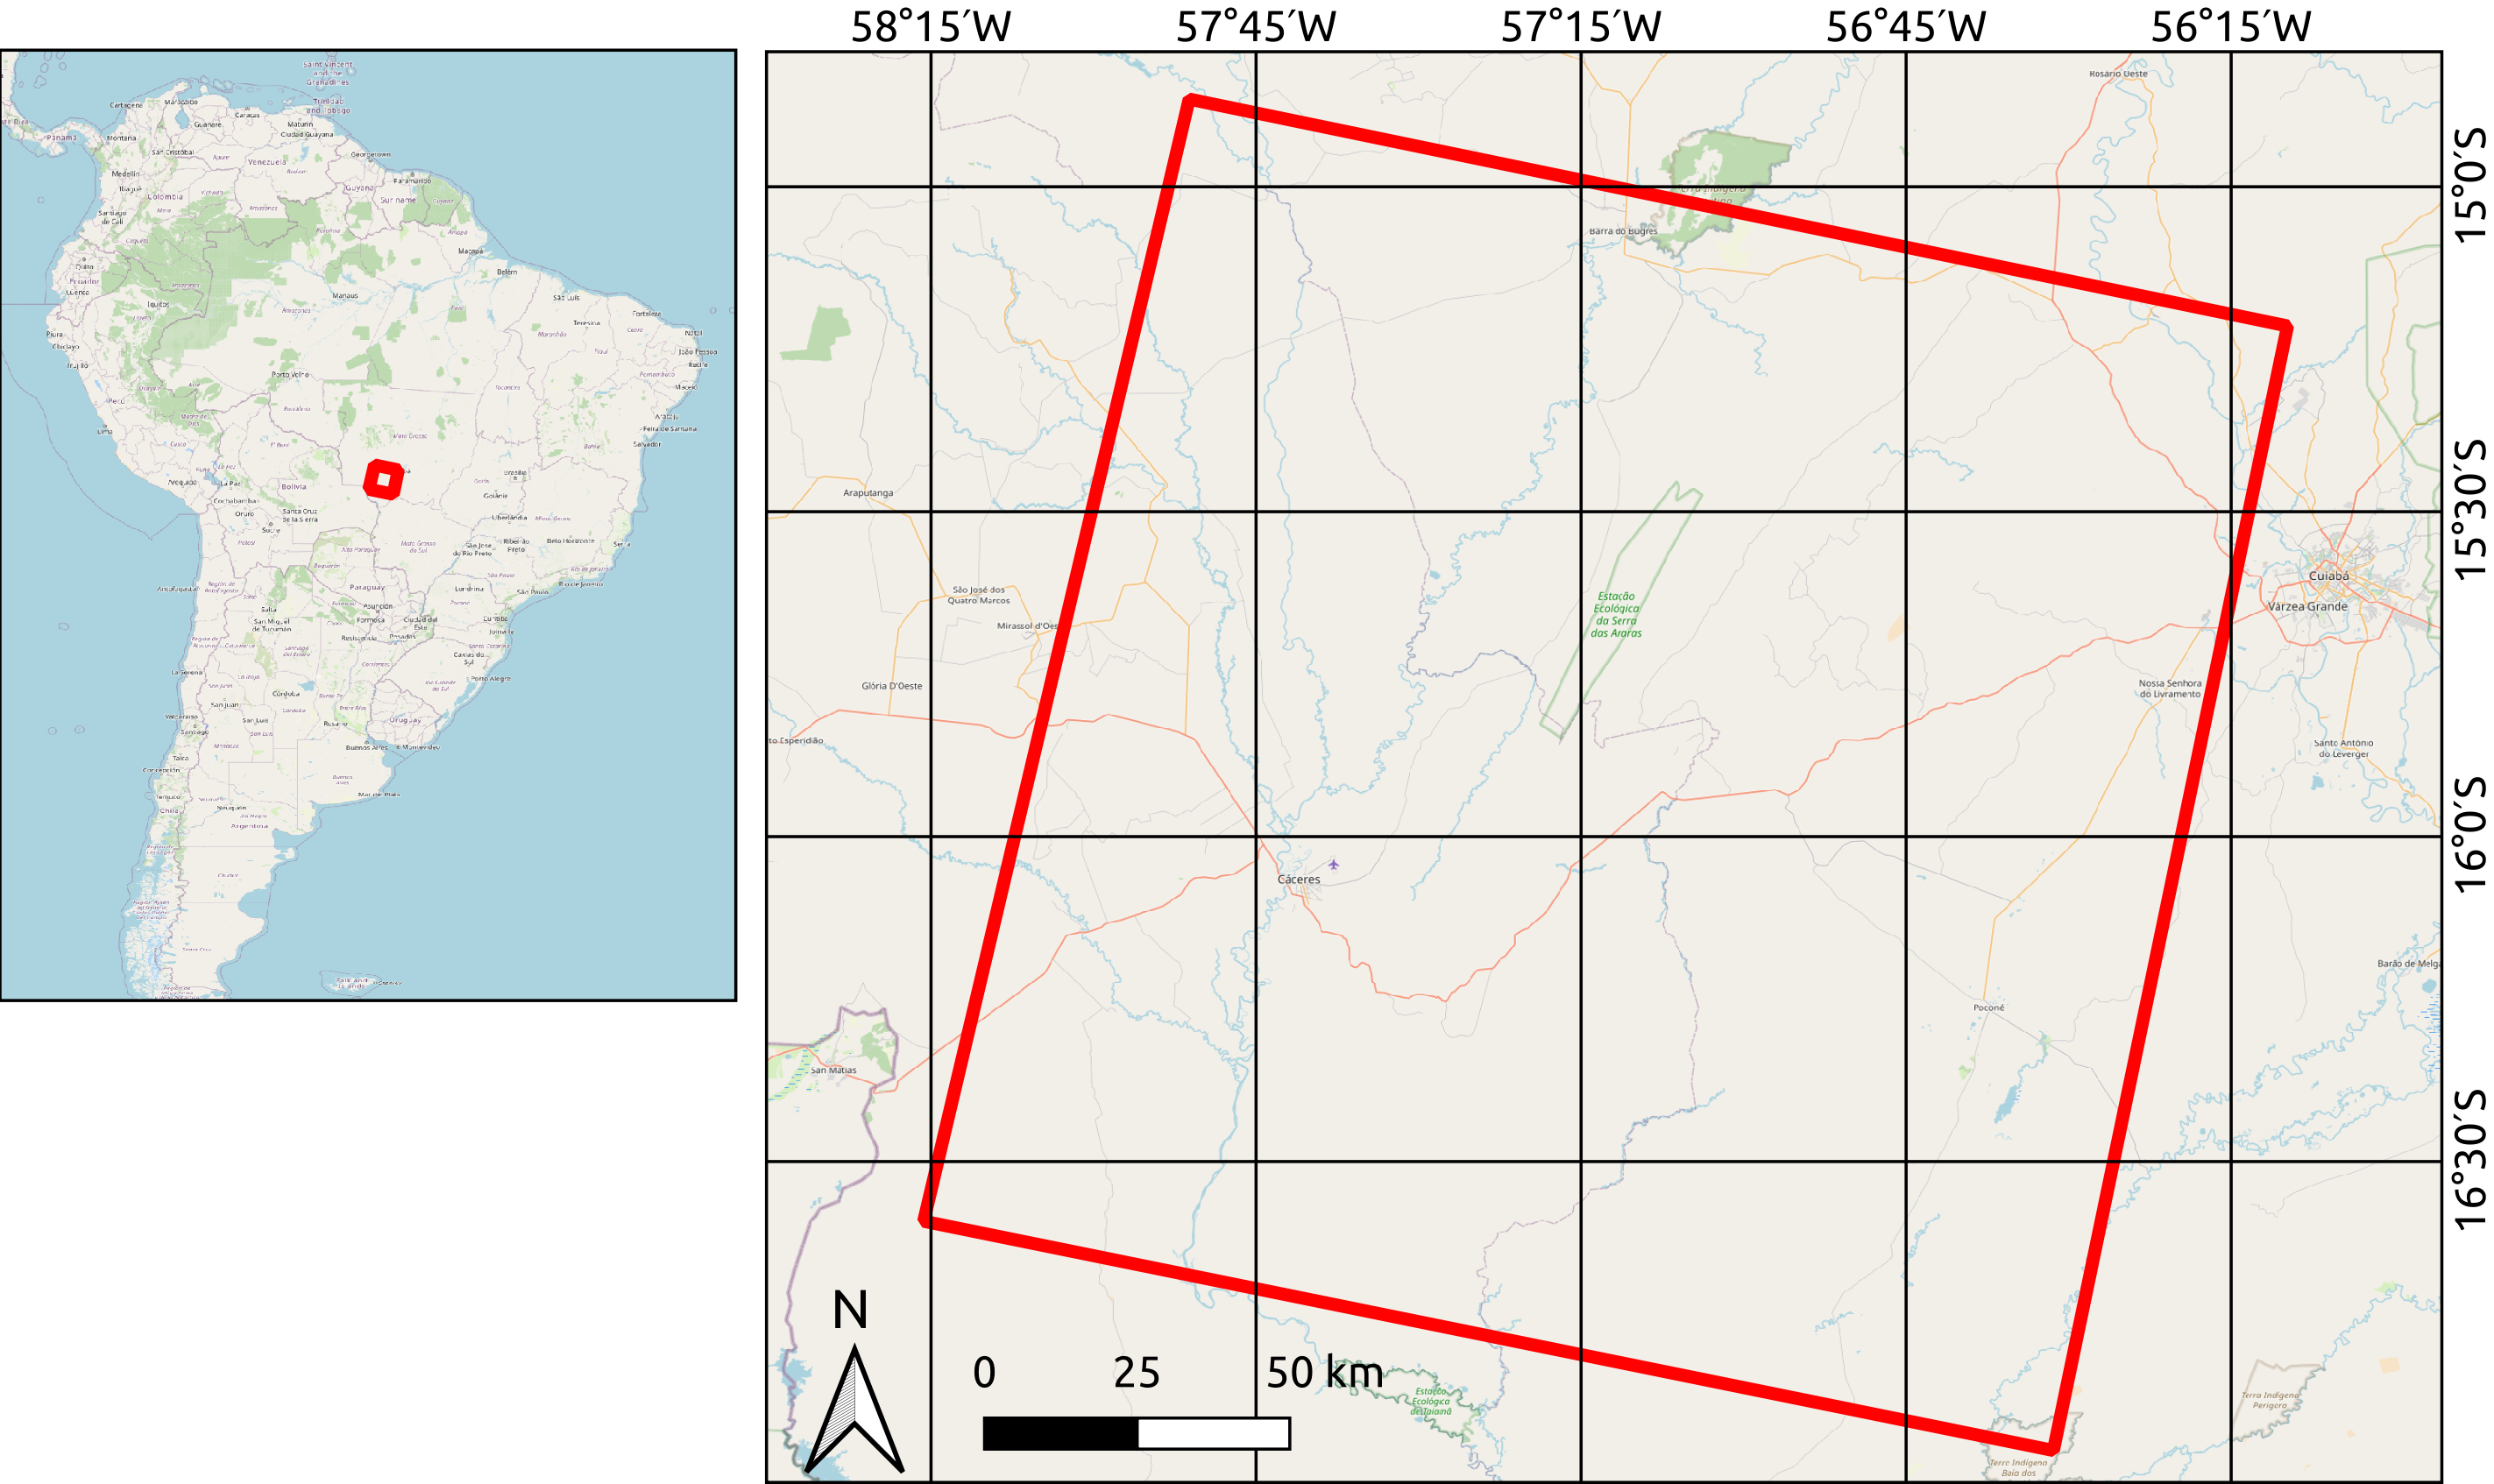
\includegraphics[width=\textwidth]{./figs/AreaEstudo.png}
\caption{�rea de estudo -- regi�o do munic�pio de C�ceres, estado do Mato-Grosso.}\label{areaestudo}
\end{figure}

%%Dados dispon�veis
Para este estudo ser� utilizada uma s�rie temporal composta por imagens dos sat�lites da s�rie LANDSAT (�ptico/multiespectral -- resolu��o espacial: $30 \ m$), referentes ao per�odo entre 2000 a 2020, disponibilizadas gratuitamente pela {\itshape United States Geological Service} -- USGS\footnote{\texttt{https://earthexplorer.usgs.gov}}.



%%%%%%%%%%%%%%%%%%%%%%%%%%%%%%%%%%%%%%%%%%%%%%%%%
\section{Ferramentas computacionais} \label{HardSoft}

Para o desenvolvimento desta pesquisa ser�o empregados o software ENVI e as linguagem de programa��o Python. O software ENVI � de grande import�ncia no aux�lio da realiza��o de tarefas gerais, por exemplo, redimensionamento e visualiza��o de imagens. A linguagem Python oferece, especialmente atrav�s das bibliotecas Numpy \cite{WaltEA2011} e Scikit-Learn \cite{PedregosaEA2011}, uma s�rie de ferramentas �teis para aplica��o de m�todos de classifica��o, regress�o ou mesmo processamento de imagens.

As ferramentas mencionadas acima assim como recursos de hardware necess�rios para a execu��o desta pesquisa estar�o � disposi��o do aluno, para acesso local ou remoto, no Laborat�rio de Inform�tica e Geoprocessamento do ICT/Unesp de S�o Jos� dos Campos.


%%%%%%%%%%%%%%%%%%%%%%%%%%%%%%%%%%%%%%%%%%%%%%%%%
\section{Plano de trabalho}

Em um primeiro momento, o projeto iniciar� com uma revis�o bibliogr�fica sobre classifica��o e regress�o de dados, em especial, envolvendo aplica��es direcionadas ao sensoriamento remoto.
Concomitantemente � revis�o bibliogr�fica citada, ser� realizado o estudo da linguagem Python e do software ENVI, necess�rios para o cumprimento das etapas seguintes.

Ainda na etapa inicial, ser�o feitas aquisi��es de imagens obtidas por sat�lites da s�rie Landsat nos anos de 2000, 2005, 2010, 2015, 2019 e 2020 com finalidade de construir uma base de dados temporal. A sele��o dos instantes em cada data est� condicionada a aus�ncia de cobertura de nuvem sobre a �rea de estudo.

Posteriormente, sobre cada um dos instantes da s�rie multitemporal, ser�o coletadas amostras de uso e cobertura do solo referentes as classes estabelecidas no escopo da proposta (Se��o~\ref{Proposta} -- i.e.; alta, m�dia e baixa biomassa, e outros). Em seguida, com uso do m�todo RF, s�o obtidas as respectivas classifica��es dos instantes da s�rie em quest�o, que posteriormente s�o usadas no c�lculo de m�tricas espaciais para express�o das din�micas locais. O processo de classifica��o e c�lculo das m�tricas espaciais ser� conduzido por fun��es implementadas em linguagem Python e com uso das bibliotecas Numpy e Scikit-Learn.

Em conson�ncia com o proposta delineada na Se��o~\ref{Proposta}, ser�o coletadas amostras sobre �reas afetadas, ou n�o, por inc�ndios a fim de construir um conjunto de dados rotulados, e que por sua vez empregado na constru��o de um modelo de regress�o log�stica. A modelagem em quest�o ser� alcan�ada com uso das mesmas ferramentas computacionais citadas anteriormente.

Em posse do modelo de regress�o, ser�o feitas extrapola��es para todas as localidades (i.e., pixels) inseridas na �rea de estudo, proporcionando assim um mapa de suscetibilidade de ocorr�ncia de inc�ndios. A avalia��o deste modelo � efetuada atrav�s da observa��o/compara��o com regi�es onde � confirmada a ocorr�ncia, ou n�o, de inc�ndio.

Por fim, a partir dos resultados, an�lises e conclus�es obtidas, ser�o redigidos o relat�rio de atividades e trabalhos para divulga��o em evento ou, se poss�vel, peri�dico cient�fico.

      %fazer

\chapter{CRONOGRAMA} \label{Cron}


Esta pesquisa ser� executada em 12 meses. As principais etapas s�o listadas abaixo e planejadas segundo o cronograma de execu��o apresentado na Tabela~\ref{cronoTab}.

%{%\singlespace

%\begin{singlespace}
\begin{enumerate}[A - ]
\item {Revis�o bibliogr�fica sobre classifica��o e regress�o de dados;} 

\item {Estudo e familiariza��o com a Linguagem Python e com o software ENVI;}

\item {Obten��o de s�rie temporal de imagens Landsat referente ao per�odo de 2000 a 2020;}

\item {Coleta de amostras sobre os tipos de uso e cobertura do solo considerados na pesquisa;}

\item {Classifica��o da s�rie temporal de imagens referente ao per�odo 2000--2019;}

\item {Implementa��o de procedimento para convers�o das classifica��es prim�rias em imagens de m�tricas espaciais;}

\item {Sele��o, em rela��o ao ano de 2020, de amostras sobre locais atingidos, ou n�o, por inc�ndios;} 

\item {Constru��o de modelo de regress�o a partir dos dados selecionados na etapa G;}

\item {Aplica��o do modelo de regress�o sobre �rea de estudo e gera��o de um mapa de suscetibilidade � inc�ndio;}

\item {An�lise dos resultados e avalia��o da acur�cia do modelo com base na imagem referente ao ano de 2020;}

\item {Reda��o de artigos cient�ficos para apresenta��o em evento ou publica��o em peri�dico;}

\item {Reda��o do relat�rio final.}
\end{enumerate}
%\end{singlespace}
%}


\begin{table}[h!]
\caption{Cronograma proposto para o desenvolvimento do projeto.} \label{cronoTab}
\centering

\begin{tabular}{|c|c|c|c|c|c|c|c|c|c|c|c|c|c|}
\cline{3-14}
\hline 
\multicolumn{2}{|c|}{M�s} & 1� & 2� & 3� & 4� & 5� & 6� & 7� & 8� & 9� & 10� & 11� & 12�\tabularnewline
\hline 
\multirow{13}{*}{\begin{sideways} Etapas \end{sideways}}  & A  & $\bullet$  & $\bullet$  &   &  &  &  &  &  &  &  &  & \tabularnewline
\cline{2-14} 
 & B  & $\bullet$  & $\bullet$  &  $\bullet$ &  &  &  &  &  &  &  &  & \tabularnewline
\cline{2-14} 
 & C  & $\bullet$  & $\bullet$  & $\bullet$ &  &  &  &  &  &  &  &  & \tabularnewline
\cline{2-14}
 & D  &   & $\bullet$  & $\bullet$ & $\bullet$ &  &  &  &  &  &  &  & \tabularnewline
\cline{2-14} 
 & E  &  & $\bullet$ & $\bullet$ & $\bullet$ &  &  &  &  &  &  &  & \tabularnewline
\cline{2-14} 
 & F  &  &  &  &  $\bullet$ &  $\bullet$ & $\bullet$ &  &  &  &  &  & \tabularnewline
\cline{2-14} 
 & G  &  &  &  &   &  & $\bullet$ & $\bullet$ & $\bullet$ &  &  &  & \tabularnewline
\cline{2-14} 
 & H  &  &  &  &  &  &  & $\bullet$ & $\bullet$ & $\bullet$ &  &  & \tabularnewline
\cline{2-14} 
 & I  &  &  &  &  &  &  &  &   & $\bullet$ & $\bullet$  &  & \tabularnewline
\cline{2-14} 
 & J  &  &  &  &  &  &  &  &   & $\bullet$ & $\bullet$  & $\bullet$ & \tabularnewline
\cline{2-14} 
 & K  &  &  &  &  &  &  &  &   & $\bullet$ & $\bullet$  & $\bullet$ & \tabularnewline
\cline{2-14} 
 & L  &  &  &  &  &  &  &  &  &  & $\bullet$ & $\bullet$ & $\bullet$ \tabularnewline
\hline 
\end{tabular}

\end{table}



%\newpage{}
  %quase...

%\newpage

\bibliography{./bib/bibNascimento__}


\inicioIndice
\end{document}